%=========================================================================
%  Simulacion de Sistemas (72.25) - Trabajo Practico Nro. 4
%  Sigue GuiaPresentaciones.pdf (las referencias "guia X.Y" apuntan ahi)
%  y las correcciones del TP3 (SdS Correcciones TP3.txt).
%=========================================================================

\documentclass[11pt,aspectratio=169]{beamer}

%------------------------- VERSION ORAL / ENTREGA (guia 2.4.8) ----------
% Entrega en campus: \vivofalse -> fotograma fijo + link a YouTube debajo.
% Exposicion en vivo: \vivotrue -> animaciones con el paquete animate (PDFs de
% fotogramas en figuras/anim_lite/; se reproducen SOLO en Adobe Acrobat Reader;
% en otros visores se ve el primer fotograma). NUNCA entregar este pdf.
\newif\ifvivo
\vivotrue

%------------------------- TEMA (guia 1.12: miniframes) -----------------
\usetheme{Berlin}
\setbeamertemplate{itemize items}[square]
\setbeamertemplate{navigation symbols}{}
\setbeamertemplate{section in toc}{\inserttocsection}   % guia 1.13: sin numerar
\setbeamercovered{invisible}

% Titulo y subtitulo CENTRADOS dentro de la barra azul.
\setbeamertemplate{frametitle}[default][center]

\setbeamersize{text margin left=1.0cm, text margin right=1.0cm}

% Pie: SOLO el numero de diapositiva (guia 1.2). Correccion TP3: no repetir
% integrantes ni numero de grupo en todas las diapositivas.
\setbeamertemplate{footline}{%
  \leavevmode\hfill
  {\usebeamerfont{page number in head/foot}%
   \usebeamercolor[fg]{structure}\insertframenumber}%
  \hspace*{0.45cm}\vskip0.22cm}

%------------------------- PAQUETES -------------------------------------
\usepackage[utf8]{inputenc}
\usepackage[T1]{fontenc}
% En Overleaf existen ambos; el IfFileExists es solo para que compile
% tambien en distribuciones minimas.
\IfFileExists{spanish.ldf}
  {\usepackage[spanish,es-noshorthands]{babel}}
  {\usepackage[main=spanish,provide=*]{babel}}
\IfFileExists{lmodern.sty}{\usepackage{lmodern}}{}
\usepackage{amsmath,amssymb}
\usepackage{graphicx}
\usepackage{booktabs}
\usepackage{algpseudocode}
\usepackage{tikz}
\usetikzlibrary{arrows.meta,positioning,calc,shapes.multipart,shadows}
\ifvivo\usepackage{animate}\fi

\graphicspath{{figuras/}}

% Links de YouTube: con la letra del texto (mas angosta que la monoespaciada) y sin
% cortar despues de "https:" (asi quedaba el link de N = 50).
\usepackage{url}
\urlstyle{same}
\def\UrlBigBreaks{}

% Pseudocodigo en castellano
\algrenewcommand\algorithmicfor{\textbf{para}}
\algrenewcommand\algorithmicdo{\textbf{hacer}}
\algrenewcommand\algorithmicif{\textbf{si}}
\algrenewcommand\algorithmicthen{\textbf{entonces}}
\algrenewcommand\algorithmicend{\textbf{fin}}

%------------------------- NOTACION (guia 3.5) --------------------------
\newcommand{\vect}[1]{\mathbf{#1}}          % vector: negrita sin italica
\newcommand{\un}[1]{\,\mathrm{#1}}          % unidad: recta
\newcommand{\sci}[2]{#1\times 10^{#2}}      % guia 1.9: potencias de 10
\newcommand{\dt}{\Delta t}
% Correccion TP3 (D26): una sola notacion para el tiempo caracteristico.
\newcommand{\tnov}{\langle t_{90}\rangle}
\newcommand{\tcien}{\langle t_{100}\rangle}
\newcommand{\kT}{k_BT}
\newcommand{\ecmE}{\mathrm{ECM}_E}           % observable de 2.1 a)

% PENDIENTE: valor o conclusion a completar con los resultados.
% Buscar "\pend" antes de entregar: no debe quedar ninguno.
% Guia 1.10: los valores con error van con las cifras significativas del error.
\newcommand{\pend}[1]{\textcolor{red}{\textbf{[#1]}}}

%------------------------- BLOQUE DE CONTENIDO CENTRADO -----------------
% Bloque centrado de ancho fijo. Soporta columns y formulas en display.
% Ajustar el ancho con el argumento opcional: \begin{cuerpo}[0.73\textwidth]
\newenvironment{cuerpo}[1][0.88\textwidth]{%
  \par\vspace{0.2em}\begin{center}\begin{minipage}{#1}}%
  {\end{minipage}\end{center}}

% Vineta cuadrada del tema para usar en renglones centrados (fuera de itemize).
\newcommand{\vineta}{\raisebox{0.2ex}{\textcolor{structure.fg}{\rule{0.42em}{0.42em}}}}

\newcommand{\cajatitulo}[1]{%
  \begin{center}%
  \begin{minipage}{0.84\textwidth}%
    \begin{beamercolorbox}[wd=\linewidth,sep=14pt,center]{title}
      \usebeamerfont{title}#1
    \end{beamercolorbox}%
  \end{minipage}%
  \end{center}}

%------------------------- FIGURAS (guia 1.7 y 1.8) ---------------------
% Guia 1.7: las figuras NO llevan titulo adentro ni caption debajo; las
% condiciones de la corrida van en el panel al costado.
% Guia 1.8 / correccion TP3: fuentes de la figura >= tamano del texto.
% Si el archivo no existe se dibuja un recuadro gris con la ruta esperada.
\newcommand{\marcador}[3]{%
  \begin{tikzpicture}
    \node[draw=gray,dashed,thick,fill=gray!8,inner sep=0pt,
          minimum width=#1,minimum height=#2,
          align=center,text=gray!60,font=\scriptsize\ttfamily]
          {figuras/\detokenize{#3}};
  \end{tikzpicture}}

% Figura con panel lateral de parametros (columna de ~0.68\textwidth)
\newcommand{\figres}[1]{%
  \IfFileExists{figuras/#1}%
    {\includegraphics[width=\linewidth,height=0.68\textheight,keepaspectratio]{figuras/#1}}%
    {\marcador{0.95\linewidth}{0.64\textheight}{#1}}}

% Fotograma (cuadrado) de una animacion
\newcommand{\fotograma}[1]{%
  \IfFileExists{figuras/#1}%
    {\includegraphics[width=\linewidth,height=0.50\textheight,keepaspectratio]{figuras/#1}}%
    {\marcador{0.48\textheight}{0.48\textheight}{#1}}}

% Animacion (guia 2.4.8; correccion TP3: maximo dos por diapositiva):
%   \figanim{fotograma.png}{video.mp4}{link}
% En el pdf de entrega: fotograma fijo y DEBAJO el link explicito.
% En vivo (\vivotrue): animacion en loop desde figuras/anim_lite/#2.pdf (5 fps).
\newcommand{\figanim}[3]{%
  \ifvivo
    \animategraphics[autoplay,loop,height=0.50\textheight]{5}{figuras/anim_lite/#2}{}{}%
  \else
    \fotograma{#1}%
  \fi
  \par\vspace{0.3em}{\scriptsize\url{#3}}}

%------------------------- PANEL DE PARAMETROS --------------------------
% Correccion TP3: aca va el numero de realizaciones (M), NUNCA la semilla.
\newcommand{\panel}[1]{%
  \begin{block}{Parámetros}
    \scriptsize
    \begin{itemize}\setlength{\itemsep}{2.5pt}#1\end{itemize}
    \vspace{2pt}
  \end{block}}

% Leyenda de colores de las animaciones (va en el panel lateral)
\newcommand{\colores}{%
  \item \textcolor{blue!75}{$\blacksquare$}~fresca,
        \textcolor{red!80!black}{$\blacksquare$}~usada,
        $\blacksquare$~obstáculo}

%------------------------- SEPARADORES DE SECCION (guia 1.13) -----------
\AtBeginSection[]{%
  \begin{frame}
    \vfill
    \cajatitulo{\insertsectionhead}
    \vfill
  \end{frame}}

%------------------------- DATOS DEL GRUPO ------------------------------
\title[Dinámica Molecular Regida por el Paso Temporal]{Trabajo Práctico N.º 4:\\ Dinámica Molecular Regida por el Paso Temporal}
\author[N. Canzonieri, L. Díaz Varela, F. Viera]{Canzonieri, Nicolás \and Díaz Varela, Lola \and Viera, Federico}
\date{2026 2C}

\begin{document}

\begin{frame}
  \vfill
  \cajatitulo{Trabajo Práctico N.º 4:\\[2pt]
    Dinámica Molecular Regida por el Paso Temporal\par
    \vskip8pt
    {\normalsize 72.25 --- Simulación de Sistemas}}

  \vskip2.2em
  \begin{center}
    {\large\textbf{2026 2C --- Grupo 9}}\par
    \vskip1.0em
    \vineta~Canzonieri, Nicolás (63501)\par
    \vskip0.45em
    \vineta~Díaz Varela, Lola (62792)\par
    \vskip0.45em
    \vineta~Viera, Federico (62022)\par
  \end{center}
  \vfill
\end{frame}
%-------------------------------------------------------------------------
%  SISTEMA 1 - UNICA diapositiva (enunciado: sin intro ni animaciones).
%  El ECM se define en el propio panel para no sumar diapositivas.
%-------------------------------------------------------------------------
\begin{frame}
  \frametitle{Comparación de Métodos Integradores}
  \framesubtitle{Oscilador Puntual Amortiguado}

  \vfill
  \begin{columns}[c]
    \begin{column}{0.62\textwidth}
      \centering
      \figres{1/ecm_vs_dt.png}
    \end{column}
    \begin{column}{0.36\textwidth}
      \begin{block}{Parámetros}
        \scriptsize
        \begin{itemize}\setlength{\itemsep}{2.5pt}
          \item $t_f=5\un{s}$
          \item $\dt$ de $10^{-6}$ a $\sci{5}{-3}\un{s}$
        \end{itemize}
      \end{block}
    \end{column}
  \end{columns}
  \vfill
\end{frame}
%=========================================================================
\section{Introducción}
%=========================================================================
% Guia 2.1: maximo 3 diapositivas. Sistema real + modelo matematico GENERAL,
% sin ningun sistema particular NI metodos de resolucion (los integradores
% van en Implementacion). Correccion TP3 (D4-D7): sin R, x0, ni m_i = m_j.

\begin{frame}
  \frametitle{Sistema Real}

  \vfill
  \begin{cuerpo}[0.80\textwidth]
    \begin{itemize}\setlength{\itemsep}{0.7em}
      \item Partículas que interactúan mediante fuerzas que dependen de las distancias entre sí.
      \item Los choques no son instantáneos.
    \end{itemize}\vspace{5pt}
    \[
        \vect{F}_i=m_i\ddot{\vect{r}}_i=\sum_{j}\vect{F}_{ij}
    \]
  \end{cuerpo}
  \vfill
\end{frame}

\begin{frame}
  \frametitle{Fundamentos}
  \framesubtitle{Resorte lineal sin fricción ni disipación}

  \vfill
  \begin{cuerpo}[0.84\textwidth]
    Colisión entre partículas:
    \[
      \vect{F}_i=\sum_{j:\ \xi_{ij}>0}-k\,\xi_{ij}\,\hat{\vect{e}}_{ij},
      \qquad
      \xi_{ij}=r_i+r_j-\left|\vect{r}_j-\vect{r}_i\right|,
      \qquad
      \hat{\vect{e}}_{ij}=\frac{\vect{r}_j-\vect{r}_i}{\left|\vect{r}_j-\vect{r}_i\right|}
    \]
    La colisión con la pared es equivalente al choque con una partícula virtual de igual radio cuyo centro se encuentra sobre la normal de contacto y a un radio de la pared.
  \end{cuerpo}
  \vfill
\end{frame}

%=========================================================================
\section{Implementación}
%=========================================================================
% Guia 2.2: solo el motor de simulacion (sin post-proceso ni formato I/O).

\begin{frame}
  \frametitle{Arquitectura del Motor}

  \vfill
  \begin{figure}[h]
  \centering
  \includegraphics[width=0.8\textwidth]{figuras/UML.jpg}
  \end{figure}
  \vfill
\end{frame}

\begin{frame}
  \frametitle{Algoritmo Implementado}

  \vfill
  \begin{center}
  \begin{minipage}{0.80\textwidth}
    \hrule height 0.4pt
    \vspace{3pt}
    {\scriptsize
    \begin{algorithmic}[1]
      \State Ubicar $N$ partículas al azar sin solapamiento, $|\vect{v}_i|=v_0$, dirección $\sim U[0,2\pi)$
      \For{$n=1,\dots,t_f/\dt$}
        \State $\vect{r}_i(t+\dt)\gets\vect{r}_i+\dt\,\vect{v}_i+\tfrac{\dt^2}{2}\vect{a}_i(t)$
        \State Armar grilla de celdas (lado $\ge 2r$) y obtener pares vecinos
        \State $\vect{a}_i(t+\dt)$: contactos partícula--partícula, partícula--obstáculo y pared (imagen)
        \State $\vect{v}_i(t+\dt)\gets\vect{v}_i+\tfrac{\dt}{2}\left[\vect{a}_i(t)+\vect{a}_i(t+\dt)\right]$
        \If{una partícula fresca tiene $\xi>0$ con un obstáculo}
          \State Marcarla usada y guardar su tiempo de conversión
        \EndIf
        \If{$n \bmod k=0$} \Comment{$\dt_2=k\,\dt$}
          \State Guardar $t$, $\vect{r}_i$, $\vect{v}_i$ y estado de cada partícula
        \EndIf
      \EndFor
    \end{algorithmic}}
    \vspace{3pt}
    \hrule height 0.4pt
  \end{minipage}
  \end{center}
  \vfill
\end{frame}

%=========================================================================
\section{Simulaciones}
%=========================================================================
% Guia 2.3: sistema particular con esquema, parametros fijos y variables,
% inputs/outputs, observables definidos matematicamente, repeticiones y
% tiempos. Correccion TP3 (D13): el esquema del sistema va en esta seccion.

% Correccion de la consulta [00:10:00-00:16:30]: Dt, el integrador y Dt2 son del
% METODO, no del sistema; van aparte y nunca entre los parametros variables.
% Consulta [00:08:15-00:17:30] y correccion TP3 (D13): el esquema va en
% Simulaciones, con los valores fijos al lado y x0 como distancia al centro.
\begin{frame}
  \frametitle{Parámetros de Simulación}
  \framesubtitle{Esquema y parámetros fijos del sistema}

  \vfill
  \begin{columns}[c]
    \begin{column}{0.46\textwidth}
      \centering
      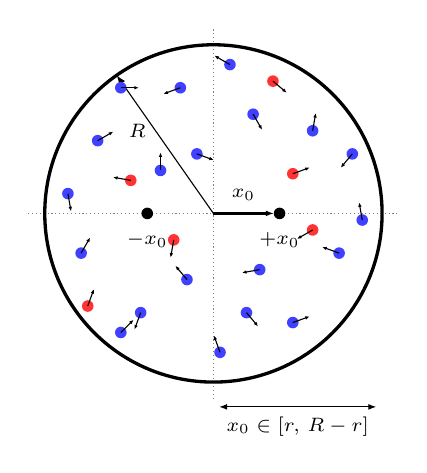
\begin{tikzpicture}[scale=4.2]
        \draw[gray,densely dotted] (-0.56,0) -- (0.56,0);
        \draw[gray,densely dotted] (0,-0.56) -- (0,0.56);
        \draw[very thick] (0,0) circle (0.51);
        \draw[-{Latex[length=1.2mm]}] (0,0) -- (125:0.51)
          node[pos=0.6,left]{\scriptsize $R$};
        % partículas frescas (a escala, r = 0.0175 m)
        \foreach \x/\y/\a in {-0.35/0.22/30, -0.10/0.38/200, 0.12/0.30/300,
                              0.30/0.25/80, 0.38/-0.12/160, 0.24/-0.33/20,
                              0.02/-0.42/110, -0.22/-0.30/250, -0.40/-0.12/60,
                              -0.05/0.18/340, 0.14/-0.17/190, -0.16/0.13/90,
                              0.42/0.18/230, -0.28/0.38/0, 0.05/0.45/150,
                              -0.44/0.06/280, -0.28/-0.36/45, 0.10/-0.30/310,
                              -0.08/-0.20/130, 0.45/-0.02/100}
          {\fill[blue!75] (\x,\y) circle (0.0175);
           \draw[-{Latex[length=0.6mm]},thin] (\x,\y) -- ++(\a:0.055);}
        % partículas usadas
        \foreach \x/\y/\a in {-0.25/0.10/170, 0.24/0.12/20, -0.12/-0.08/260,
                              0.18/0.40/320, -0.38/-0.28/70, 0.30/-0.05/210}
          {\fill[red!80] (\x,\y) circle (0.0175);
           \draw[-{Latex[length=0.6mm]},thin] (\x,\y) -- ++(\a:0.055);}
        % obstáculos fijos
        \fill (-0.20,0) circle (0.0175);
        \fill ( 0.20,0) circle (0.0175);
        \node[below=1pt,font=\scriptsize] at (-0.20,-0.02) {$-x_0$};
        \node[below=1pt,font=\scriptsize] at ( 0.20,-0.02) {$+x_0$};
        % x0: distancia del centro del recinto al centro de un obstáculo
        \draw[-{Latex[length=1mm]},thick] (0,0) -- (0.1825,0)
          node[midway,above=1pt,font=\scriptsize]{$x_0$};
        % rango de x0
        \draw[{Latex[length=1mm]}-{Latex[length=1mm]},thin] (0.0175,-0.585) -- (0.4925,-0.585)
          node[midway,below,font=\scriptsize]{$x_0\in[r,\,R-r]$};
      \end{tikzpicture}\par\vspace{0.2em}
      {\scriptsize \textcolor{blue!75}{$\blacksquare$}~fresca\quad
       \textcolor{red!80}{$\blacksquare$}~usada\quad $\blacksquare$~obstáculo}
    \end{column}
    \begin{column}{0.50\textwidth}
      \centering
      \scriptsize
      \renewcommand{\arraystretch}{1.08}
      \begin{tabular}{@{}l@{\hspace{0.8em}}l@{\hspace{1.0em}}l@{}}
        \toprule
        \textbf{Símbolo} & \textbf{Valor} & \textbf{Descripción}\\
        \midrule
        $R$   & $0.51\un{m}$     & Radio del recinto\\
        $r$   & $\sci{1.75}{-2}\un{m}$    & Radio de partículas y obstáculos\\
        $m$   & $\sci{2.5}{-2}\un{kg}$    & Masa de las partículas\\
        $k$   & $10^{4}\un{N/m}$          & Constante del resorte de contacto\\
        $v_0$ & $1\un{m/s}$               & Módulo de la velocidad inicial\\
        \bottomrule
      \end{tabular}
      \vspace{0.8em}
    \end{column}
  \end{columns}
  \vfill
\end{frame}

\begin{frame}
  \frametitle{Parámetros de Simulación}
  \framesubtitle{Parámetros variables del sistema}

  \vfill
  \begin{center}
    \scriptsize
    \renewcommand{\arraystretch}{1.15}
    \begin{tabular}{@{}l l l l l l@{}}
      \toprule
      \textbf{Estudio} & \textbf{Obstáculos} & $\boldsymbol{N}$ & $\boldsymbol{t_f}$ & $\boldsymbol{M}$ & \textbf{Parámetro variable}\\
      \midrule
      Paso temporal & no & $300$ & $30\un{s}$ & $10$ & $\Delta t$\\
      Número de partículas & $x_0=r$                     & $5$ a $650$    & $30\un{s}$     & $10$ & $N$\\
      Densidad, $t_f$ largo & $x_0=r$                    & $5$ a $200$    & $10^{2}\un{s}$ & $10$ & $N$\\
      Posición obstáculos  & $x_0\in[r,R-r]$, 9 valores  & $100$ y $20$   & $10^{2}\un{s}$ & $5$  & $x_0$\\
      Mapa de calor        & $x_0\in[r,R-r]$, 7 valores  & $20$ a $200$   & $10^{2}\un{s}$ & $3$  & $(x_0,N)$\\
      Velocidades          & no                          & $100$          & $10\un{s}$     & $10$ & --- (evolución temporal)\\
      \bottomrule
    \end{tabular}

    \vspace{0.9em}
    % Correccion TP2 (D15): la notacion se introduce aca, no en los observables.
    \begin{tabular}{@{}r@{\hspace{0.6em}}p{0.72\textwidth}@{}}
      \textbf{$M$:}      & realizaciones independientes por configuración\\
      \textbf{Densidad:} & $\rho=N/(\pi R^2)$\\
      \textbf{Output:}   & $t$, $\vect{r}_i$, $\vect{v}_i$ y estado de cada partícula cada $\dt_2$;
                           tiempo de conversión de cada partícula
    \end{tabular}
  \end{center}
  \vfill
\end{frame}

% Guia 2.3: observables definidos matematicamente y como se promedia.
% Guia 1.6 y correccion TP2 (D15): poco texto. Solo las definiciones propias
% (F_u, t90 y f_MB ya estan en el enunciado); el resto va a NOTAS.md.
% Energia: como physics.py (kinetic_energy, potential_energy): 1/2 m v^2 y
% 1/2 k xi^2 por cada contacto con xi > 0 (pares, obstaculos y pared imagen).
\begin{frame}
  \frametitle{Observables}
  \framesubtitle{Energía y su ECM}

  \vfill
  \begin{center}
    \textbf{Energía total del sistema en $t$}
    \[
      E(t)=\frac{1}{2}\,m\sum_{i=1}^{N}\left|\vect{v}_i(t)\right|^2
      +\frac{k}{2}\sum_{\xi>0}\xi^2(t)
    \]
    {\footnotesize Suma sobre todos los contactos: partícula--partícula y partícula--pared.}\par
    \vspace{1.5em}
    \textbf{Error Cuadrático Medio de la Energía}
    \[
      \ecmE=\frac{1}{N_t}\sum_{n=1}^{N_t}\left[E(t_n)-E(0)\right]^2
    \]
  \end{center}
  \vfill
\end{frame}

% Guia 2.3 y correccion TP2 (D15): explicitar como se promedia y el desvio
% estandar con M - 1 (varias realizaciones).
\begin{frame}
  \frametitle{Observables}
  \framesubtitle{Tiempos característicos y promedios}

  \vfill
  \begin{center}
    \textbf{Tiempos característicos}
    \[
      t_{90}=\min\{t:\ F_u(t)\ge 0.9\},
      \qquad
      t_{100}=\min\{t:\ F_u(t)=1\}
    \]
    \textbf{Promedio sobre $M$ realizaciones}
    \[
      \langle X\rangle=\frac{1}{M}\sum_{q=1}^{M}X^{(q)},
      \qquad
      \sigma_X=\sqrt{\frac{1}{M-1}\sum_{q=1}^{M}\left(X^{(q)}-\langle X\rangle\right)^2}
    \]
  \end{center}
  \vfill
\end{frame}

% Guia 2.4.5 y correccion TP3 (D30): el ajuste minimiza el error E; la figura de
% E(kT) se muestra en Resultados.
\begin{frame}
  \frametitle{Observables}
  \framesubtitle{Distribución de velocidades}

  \vfill
  \begin{center}
    \textbf{Distribución del módulo de la velocidad}
    \[
      f(v_j,t)=\frac{n_j(t)}{M\,N\,\Delta v}
    \]
    \vspace{0.8em}
    \textbf{Ajuste de Maxwell-Boltzmann}
    \[
      E(\kT)=\sum_j\left[f(v_j)-f_{\mathrm{MB}}(v_j;\kT)\right]^2,
      \qquad
      \kT^{*}=\arg\min_{\kT}E(\kT)
    \]
  \end{center}
  \vfill
\end{frame}

%=========================================================================
\section{Resultados}
%=========================================================================
% Guia 2.4: para cada input -> animacion (1 o 2 extremos) -> evolucion
% temporal (solo valores extremos) y el escalar que la caracteriza ->
% input vs observable con promedio y barras de error.
% Primero la puesta a punto del metodo (Dt, 2.1 a; no es input del sistema).
% Orden de los ejercicios: 2.1 a, 2.1 b, 2.2, 2.3, 2.4 a, 2.4 b. Dentro de cada uno,
% animacion -> evolucion temporal -> observable (guia 2.4.1-2.4.4).

%-------------------------------------------------------------------------
%  PUESTA A PUNTO DEL METODO: ELECCION DE Dt (2.1 a)
%  Dt NO es un input del sistema (consulta [00:10:00-00:16:30]): se ajusta
%  antes de estudiar el billar y queda fijo en todo lo que sigue.
%-------------------------------------------------------------------------
% Sin animacion propia: el sistema sin obstaculos ya se anima en 2.3 y con
% cualquier dt aceptable se ve igual (correccion: no repetir lo mismo con otra N).
\begin{frame}
  \frametitle{Elección del Paso Temporal}
  \framesubtitle{Observable: Evolución de la Energía según $\Delta t$}

  \vfill
  \begin{columns}[c]
    \begin{column}{0.66\textwidth}
      \centering
      \figres{2.1a/energy_vs_time.png}
    \end{column}
    \begin{column}{0.30\textwidth}
      \panel{\item Sin obstáculos, $N=300$
             \item $t_f=30\un{s}$
             \item Una realización}
    \end{column}
  \end{columns}
  \vfill
\end{frame}

\begin{frame}
  \frametitle{Elección del Paso Temporal}
  \framesubtitle{Observable: $\langle\ecmE\rangle$ en función de $\dt$}

  \vfill
  \begin{columns}[c]
    \begin{column}{0.66\textwidth}
      \centering
      \figres{2.1a/energy_observable_vs_dt.png}
    \end{column}
    \begin{column}{0.30\textwidth}
      \panel{\item Sin obstáculos, $N=300$
             \item $t_f=30\un{s}$
             \item $M=10$
             \item $\dt$ elegido: $10^{-4}\un{s}$}
    \end{column}
  \end{columns}
  \vfill
\end{frame}

%-------------------------------------------------------------------------
%  2.1 b) TIEMPO DE EJECUCION EN FUNCION DE N
%-------------------------------------------------------------------------
\begin{frame}
  \frametitle{Tiempo de Ejecución}
  \framesubtitle{Observable: Tiempo de ejecución en función de $N$}

  \vfill
  \begin{columns}[c]
    \begin{column}{0.66\textwidth}
      \centering
      \figres{2.1b/runtime_vs_n_log.png}
    \end{column}
    \begin{column}{0.30\textwidth}
      \panel{\item $x_0=r$
             \item $t_f=30\un{s}$
             \item $M=10$}
    \end{column}
  \end{columns}
  \vfill
\end{frame}

%-------------------------------------------------------------------------
%  2.2) POSICION DE LOS OBSTACULOS
%-------------------------------------------------------------------------
\begin{frame}
  \frametitle{Posición de los Obstáculos}
  \framesubtitle{Animaciones}

  \vfill
  \begin{columns}[t]
    \begin{column}{0.36\textwidth}
      \centering
      \textbf{$x_0=R/2$}\par\vspace{0.3em}
      \figanim{2.2/configuracion_N=100_x0=0.2550.png}{x0_R2}{https://youtube.com/shorts/dKyPh__Wdps?si=QRQzofiYVgCwGk3M}
    \end{column}
    \begin{column}{0.36\textwidth}
      \centering
      \textbf{$x_0=R-r$}\par\vspace{0.3em}
      \figanim{2.2/configuracion_N=100_x0=0.4925.png}{x0_Rr}{https://youtube.com/shorts/ch0G7yJCVGk?si=9dNg3wqv99IItuBE}
    \end{column}
    \begin{column}{0.24\textwidth}
      \panel{\item $N=100$
             \item $t_f=10^{2}\un{s}$
             \item Una realización}
    \end{column}
  \end{columns}
  \vfill
\end{frame}

\begin{frame}
  \frametitle{Posición de los Obstáculos}
  \framesubtitle{Observable: Evolución de $\langle F_u(t)\rangle$}

  \vfill
  \begin{columns}[c]
    \begin{column}{0.66\textwidth}
      \centering
      \figres{2.2/fu_vs_time_N=100.png}
    \end{column}
    \begin{column}{0.30\textwidth}
      \panel{\item $N=100$
             \item $x_0=r$, $\sci{2.55}{-1}\un{m}$ y $R-r$
             \item $t_f=10^{2}\un{s}$
             \item $M=5$}
    \end{column}
  \end{columns}
  \vfill
\end{frame}

% Enunciado 2.2: comparar el resultado FINAL con menor densidad (N = 20).
% Una sola diapo: la curva de N = 100 ya esta superpuesta con la de N = 20.
\begin{frame}
  \frametitle{Posición de los Obstáculos}
  \framesubtitle{Observable: $\tnov$ en función de $x_0$ para dos densidades}

  \vfill
  \begin{columns}[c]
    \begin{column}{0.66\textwidth}
      \centering
      \figres{2.2/t90_vs_x0.png}
    \end{column}
    \begin{column}{0.30\textwidth}
      \panel{\item $N=100$ y $N=20$
             \item 9 posiciones entre $r$ y $R-r$
             \item $t_f=10^{2}\un{s}$
             \item $M=5$}
    \end{column}
  \end{columns}
  \vfill
\end{frame}

% Solo si alguna realizacion no alcanza F_u = 0.9 antes de t_f
% (el estudio genera 2.2/fu_tmax_vs_x0.png en ese caso).
% \begin{frame}
%   \frametitle{Posición de los Obstáculos}
%   \framesubtitle{Observable: $\langle F_u(t_f)\rangle$ en función de $x_0$}
%   \vfill
%   \begin{columns}[c]
%     \begin{column}{0.66\textwidth}
%       \centering
%       \figres{2.2/fu_tmax_vs_x0.png}
%     \end{column}
%     \begin{column}{0.30\textwidth}
%       \panel{\item $N=100$ y $N=20$
%              \item $t_f=10^{2}\un{s}$
%              \item $M=5$}
%     \end{column}
%   \end{columns}
%   \vfill
% \end{frame}

%-------------------------------------------------------------------------
%  DISTRIBUCION DE VELOCIDADES (2.3)
%-------------------------------------------------------------------------
\begin{frame}
  \frametitle{Distribución de Velocidades}
  \framesubtitle{Animación}

  \vfill
  \begin{columns}[c]
    \begin{column}{0.50\textwidth}
      \centering
      \figanim{2.3/anim_N100_sin_obstaculos.png}{vel}{https://youtube.com/shorts/-WK5T7Y3pEo?si=SjeUTBD9aTdeug8A}
    \end{column}
    \begin{column}{0.36\textwidth}
      \panel{\item Sin obstáculos
             \item $N=100$
             \item $t_f=2\un{s}$
             \item Una realización}
    \end{column}
  \end{columns}
  \vfill
\end{frame}

\begin{frame}
  \frametitle{Distribución de Velocidades}
  \framesubtitle{Observable: Evolución de $f(v,t)$}

  \vfill
  \begin{columns}[c]
    \begin{column}{0.66\textwidth}
      \centering
      \figres{2.3/fv_vs_time.png}
    \end{column}
    \begin{column}{0.30\textwidth}
      \panel{\item Sin obstáculos, $N=100$
             \item $M=10$, $\dt_2=10^{-2}\un{s}$}
    \end{column}
  \end{columns}
  \vfill
\end{frame}

% Guia 2.4.5 y correccion TP3 (D30): mostrar como se hallo el mejor ajuste.
% Consulta [01:49:30-01:51:30]: f(v,t) -> como se ajusta -> estacionario.
\begin{frame}
  \frametitle{Distribución de Velocidades}
  \framesubtitle{Ajuste: Error en función de $\kT$}

  \vfill
  \begin{columns}[c]
    \begin{column}{0.66\textwidth}
      \centering
      \figres{2.3/fit_error.png}
    \end{column}
    \begin{column}{0.30\textwidth}
      \panel{\item Sin obstáculos, $N=100$
             \item $M=10$, $\dt_2=10^{-2}\un{s}$}
    \end{column}
  \end{columns}
  \vfill
\end{frame}

\begin{frame}
  \frametitle{Distribución de Velocidades}
  \framesubtitle{Búsqueda del Estacionario: Ajuste de cada $f(v,t)$}

  \vfill
  \begin{columns}[c]
    \begin{column}{0.66\textwidth}
      \centering
      \figres{2.3/stationarity.png}
    \end{column}
    \begin{column}{0.30\textwidth}
      \panel{\item Sin obstáculos, $N=100$
             \item $M=10$, $\dt_2=10^{-2}\un{s}$}
    \end{column}
  \end{columns}
  \vfill
\end{frame}

\begin{frame}
  \frametitle{Distribución de Velocidades}
  \framesubtitle{Distribución Estacionaria y Ajuste}

  \vfill
  \begin{columns}[c]
    \begin{column}{0.66\textwidth}
      \centering
      \figres{2.3/fv_stationary_fit.png}
    \end{column}
    \begin{column}{0.30\textwidth}
      \panel{\item Sin obstáculos, $N=100$
             \item $M=10$, $\dt_2=10^{-2}\un{s}$}
    \end{column}
  \end{columns}
  \vfill
\end{frame}

%-------------------------------------------------------------------------
%  2.4 a) EFECTO DE LA DENSIDAD (mismas corridas que 2.1 b)
%  Animaciones de N aca: muestran la conversion que miden F_u y t90.
%-------------------------------------------------------------------------
\begin{frame}
  \frametitle{Efecto de la Densidad}
  \framesubtitle{Animaciones}

  \vfill
  \begin{columns}[t]
    \begin{column}{0.36\textwidth}
      \centering
      \textbf{$N=50$}\par\vspace{0.3em}
      \figanim{2.4a/anim_N50.png}{N50}{https://youtube.com/shorts/wMe-19TIZv4}
    \end{column}
    \begin{column}{0.36\textwidth}
      \centering
      \textbf{$N=650$}\par\vspace{0.3em}
      \figanim{2.4a/anim_N650.png}{N650}{https://youtube.com/shorts/XU6uyWSFlnQ?si=KBOxyNv9hVzCfq_k}
    \end{column}
    \begin{column}{0.24\textwidth}
      \panel{\item $x_0=r$
             \item $t_f=30\un{s}$
             \item Una realización}
    \end{column}
  \end{columns}
  \vfill
\end{frame}

% Guia 2.4: animacion -> evolucion temporal -> escalares. Densidad baja,
% optima y alta (curve_ns de density.py).
\begin{frame}
  \frametitle{Efecto de la Densidad}
  \framesubtitle{Observable: Evolución de $\langle F_u(t)\rangle$}

  \vfill
  \begin{columns}[c]
    \begin{column}{0.66\textwidth}
      \centering
      \figres{2.4a/fu_vs_time.png}
    \end{column}
    \begin{column}{0.30\textwidth}
      \panel{
             \item $x_0=r$, $t_f=30\un{s}$
             \item $M=10$}
    \end{column}
  \end{columns}
  \vfill
\end{frame}

\begin{frame}
  \frametitle{Efecto de la Densidad}
  \framesubtitle{Observable: $\langle F_u(t_f)\rangle$ en función de la densidad}

  \vfill
  \begin{columns}[c]
    \begin{column}{0.66\textwidth}
      \centering
      \figres{2.4a/fu_tf_vs_density.png}
    \end{column}
    \begin{column}{0.30\textwidth}
      \panel{\item $N=5$ a $650$
             \item $x_0=r$, $t_f=30\un{s}$
             \item $M=10$}
    \end{column}
  \end{columns}
  \vfill
\end{frame}

\begin{frame}
  \frametitle{Efecto de la Densidad}
  \framesubtitle{Observable: $\tnov$ y $\tcien$ en función de la densidad}

  \vfill
  \begin{columns}[c]
    \begin{column}{0.66\textwidth}
      \centering
      \figres{2.4a/t_vs_density.png}
    \end{column}
    \begin{column}{0.30\textwidth}
      \panel{\item $N=5$ a $200$
             \item $x_0=r$, $t_f=30\un{s}$
             \item $M=10$}
    \end{column}
  \end{columns}
  \vfill
\end{frame}

% Corrida complementaria: con t_f = 30 s (impuesto por 2.1 b) los umbrales no
% se alcanzan a baja ni a alta densidad; con t_f = 100 s todas llegan a 0.9 y
% solo t100 tiene realizaciones censuradas (N = 10 y 200).
\begin{frame}
  \frametitle{Efecto de la Densidad}
  \framesubtitle{Observable: $\tnov$ y $\tcien$ en función de la densidad, $t_f=10^{2}\un{s}$}

  \vfill
  \begin{columns}[c]
    \begin{column}{0.66\textwidth}
      \centering
      \figres{2.4a/t_vs_density_tf100.png}
    \end{column}
    \begin{column}{0.30\textwidth}
      \panel{\item $N=5$ a $200$
             \item $x_0=r$, $t_f=10^{2}\un{s}$
             \item $M=10$}
    \end{column}
  \end{columns}
  \vfill
\end{frame}

%-------------------------------------------------------------------------
%  2.4 b) (opcional) POSICION OPTIMA PARA DISTINTAS DENSIDADES
%-------------------------------------------------------------------------
% 2.4 b) (opcional): x0 optimo para distintas densidades.
\begin{frame}
  \frametitle{Posición de los Obstáculos}
  \framesubtitle{Observable: $\tnov$ en función de $(x_0,N)$}

  \vfill
  \begin{columns}[c]
    \begin{column}{0.68\textwidth}
      \centering
      \figres{2.4b/heatmap_t90.png}
    \end{column}
    \begin{column}{0.28\textwidth}
      \panel{\item $N=20$ a $200$
             \item 7 posiciones entre $r$ y $R-r$
             \item $t_f=10^{2}\un{s}$
             \item $M=3$}
    \end{column}
  \end{columns}
  \vfill
\end{frame}

%=========================================================================
\section{Conclusiones}
%=========================================================================
% Guia 2.5: UNA diapositiva, basada SOLO en resultados mostrados; sin
% hipotesis no estudiadas ni tareas pendientes.

\begin{frame}
  \frametitle{Conclusiones}
  \framesubtitle{Resumen de resultados}

  \vfill
  \begin{cuerpo}[0.92\textwidth]
    \small
    \begin{itemize}\setlength{\itemsep}{0.45em}
      \item Oscilador: \textbf{Beeman es el integrador más preciso} en todo el rango de $\dt$.
      \item Se halló un \textbf{paso temporal máximo que conserva la energía}. Por encima, la energía diverge.
      \item \textbf{Por Eventos conviene en sistemas diluidos y Paso Temporal en densos}:
            el costo de eventos crece cada vez más rápido con $N$; el de paso temporal, linealmente.
      \item Con los obstáculos en el centro se halló una \textbf{densidad óptima}:
            con menos o más partículas, $\langle F_u(t)\rangle$ crece más despacio.
      \item $\tnov$ es \textbf{mínimo con los obstáculos a distancia intermedia} del centro.
            A menor densidad, esa zona es más ancha.
      \item La distribución estacionaria es \textbf{Maxwell-Boltzmann}, con $\kT^{*}$ compatible con $m v_0^2/2$.
    \end{itemize}
  \end{cuerpo}
  \vfill
\end{frame}

\begin{frame}
  \vfill
  \cajatitulo{¡Muchas Gracias!}
  \vfill
\end{frame}


\begin{frame}
  \frametitle{Disclaimer}
  \framesubtitle{Uso de inteligencia artificial}

  \vfill
  \begin{cuerpo}[0.84\textwidth]
    \begin{itemize}\setlength{\itemsep}{0.8em}
      \item Usamos Claude Opus 5.5 (Medium y High) como asistente de programación.
      \item Con él escribimos e iteramos el código del motor y del
            post-procesamiento, a partir del material de la cátedra:
            enunciado, Teórica 4 y guía de presentaciones.
      \item Cada cambio fue revisado y verificado por el equipo
      \item Todas las decisiones de modelado, parámetros, observables e
            interpretación de resultados las tomó el equipo: la IA nunca
            decidió por sí sola. Simplemente fue prompteada a implementar las propuestas del equipo.
    \end{itemize}
  \end{cuerpo}
  \vfill
\end{frame}

\end{document}
